\documentclass[10pt,letterpaper]{article}

\usepackage{cogsci}
\usepackage{pslatex}
\usepackage[nodoi]{apacite}
\usepackage{graphicx}
\usepackage[american]{babel}
\usepackage{amsmath}
\usepackage[section]{placeins}
\usepackage{enumitem}
\usepackage{tikz}
\usetikzlibrary{bayesnet}

\setlength{\textfloatsep}{12pt plus 1.0pt minus 2.0pt}

\title{Linguistic input is tuned to children's developmental level}

 \author{{\large \bf Daniel Yurovsky} \\ \texttt{yurovsky@stanford.edu}\\ Department of Psychology \\ Stanford University
 	\And {\large \bf Gabriel Doyle} \\ \texttt{gdoyle@stanford.edu} \\ Department of Psychology \\ Stanford University
	\And {\large \bf Michael C. Frank} \\ \texttt{mcfrank@stanford.edu} \\ Department of Psychology \\ Stanford University}

\begin{document}

\maketitle

\begin{abstract}

\vspace{-6 pt}Children rapidly learn a tremendous amount about language despite limitations imposed on them by their developing cognitive abilities. One possible explanation for this rapid learning is that caregivers tune the language they produce to these limitations, titrating the complexity of their speech to developmentally-appropriate levels. We test this hypothesis in a large-scale corpus analysis, measuring the contingency between parents' and children's speech over the first 5 years. Our results support the linguistic tuning hypothesis, showing a high degree of mostly parent-led coordination early in development that decreases as children become more proficient language learners and users.

\textbf{Keywords:}
Language acquisition, cognitive development, computational models
\end{abstract}

\section{Introduction}

Children acquire a tremendous amount of language in their first few years of life. By the time they are able to run down the street, typically developing children have over a thousand words in their productive vocabularies \cite{mayor2011}. They can combine these words to produce new, meaningful multi-word utterances \cite{lieven2009}. They can even learn new words from just the syntactic constructions in which they occur \cite{yuan2009}. What explains this rapid developmental progression?

Young children have access to a surprising range of learning mechanisms. By 8-months, infants can use distributional properties of language to segment discrete words from continuous speech \cite{saffran1996}, and by 12 months can use these same kinds of cues to learn ordering regularities in artificial grammars \cite{gomez1999} and mappings between words and objects \cite{smith2008}. But while these and other competencies are available early, the amount of information that children can actually learn in lab experiments often strikingly limited. For instance, children's learning of new words from distributional properties of language is highly constrained by their developing attentional and memory systems \cite{vlach2013}.

How can children learn so quickly when their learning abilities are so constrained? One possibility is that the speech that children hear in the world differs systematically from speech used to test their learning in the laboratory. Indeed, the language that parents produce to their children---across a variety of levels and structures---appears to contain many redundant cues that facilitate learning \cite{gogate2000, thiessen2005, yurovsky2012}. However, in some cases child-directed speech appears systematically different in ways that do not support learning. For instance, child-directed speech typically contains simpler and less variable syntactic structures. This simplicity helps children learn simple structures, but also makes it harder for them to learn more complex ones \cite{montag2015a, montag2015b}. The input that is best for children's learning thus depends on what they already know, and what they are trying to learn next.

The explanation for rapid language acquisition may thus be neither in the learner nor in the input, but in the coordination between learner and input: Parents may tune the complexity of their language to the developing abilities and needs of their children. This \emph{linguistic tuning} hypothesis is intuitively appealing, and was supported by some early evidence \cite{snow1972}. However, two pieces of contradictory evidence diminished initial enthusiasm for it. First, parents do not appear to use simpler words when speaking to younger children \cite{hayes1988}. Second, parents rarely show sensitivity to their children's syntactic errors by correcting them, and children are resistant to the few corrections they get \cite{brown1970, newport1977}.

More recent work has suggested other---perhaps more subtle---ways in which parents might tune the language they produce in response to children's developing knowledge and learning mechanisms. Although they do not correct syntactic errors, parents are much more likely to repeat and reformulate children's ungrammatical utterances, providing a potential corrective signal \cite{hirsh-pasek1984, chouinard2003}. And although parents' vocabulary choices may be due at least in part to the content they need to convey, there may still be ways for adults to tailor the structure of their utterances to children's perceived competence. In the current paper, we pursue this question, asking whether parents choose their non-content words in a manner contingent on their children's developmental level.

To test whether parents tune their speech to that of their children, we conduct a large-scale corpus study using \emph{linguistic alignment}, a measure of how much speakers change the way they talk to accommodate their conversational partners. Critically, alignment is a local measure: High alignment results not from choosing words that are simpler overall, but from choosing words that are more contingent on one's conversational partner, and thus easier to process in context \cite<cf.>{hayes1988}. We predict that caregivers should alter their levels of alignment across development, aligning more to younger children who need more linguistic support.

\subsection{Linguistic alignment}

When we use language to communicate, we use the words we say to convey the message we intend. Some of these words will be critical for getting the message across. Consider the conversation in Table~\ref{tab:naima}, taken from the Providence corpus \cite{demuth2006}. In her first response, Naima's mom has little choice but to say ``sweet potato'' if she wants to inform Naima that they are eating sweet potato. However, she could perfectly well have left out the words ``some,'' ``that,'' and ``this,'' or exchanged them for others and still conveyed the identity of the food on Naima's plate.

\begin{table}[tb]
\begin{tabular}{r p{.35\textwidth}}
\hline
Naima: & Eating \textbf{that}. Eating \textbf{some of that}.\\

Mom: & \textbf{Some of this}? \textbf{You} know what \textbf{that} is? \textbf{It} is sweet potato.\\

Naima: & \textbf{I} am \textbf{a} bear \textbf{that} eats.\\

Mom: & \textbf{You're a} bear \textbf{that} eats what? What do \textbf{you} eat little bear?\\

Naima: & Fresh pear\\
\hline
\end{tabular}
\caption{\label{tab:naima} An exchange between Naima (20-mo.) and her mom in the Providence Corpus. Bolded words are LIWC category members included in the model \cite{pennebaker2007}. }
\end{table}

Speakers are influenced in their production choices by a variety of factors, ranging from the phonological to the sociolinguistic. We focus here one particular reason for these choices: Contingency on a conversational partner. When we talk, we tend to re-use use each-other's expressions, aligning to each other. This kind of alignment appears to be a pervasive property of human social interaction and linguistic communication \cite{giles1991, garrod2004}. Further, alignment appears to be useful, facilitating fluent processing of speech, and increasing the probability of successful communication and accomplishment of joint goals \cite{ireland2011, fusaroli2012}. Critically, alignment is directional: Even in the same conversation, some speakers will align more than others. For instance, alignment varies across a social hierarchy, with less powerful speakers aligning more to powerful speakers \cite{kacewicz2013}. Thus, linguistic alignment can measure a speaker's effort to  coordinate with a conversational partner. We leverage this property to measure the extent to which parents are altering the way they speak to coordinate with their developing children.

We explicitly focus on the words that are least critical for conveying the content of the message. If Mom produces ``sweet potato'' after Naima does, we know only that they are discussing the same object. However, if Mom produces a function word like ``of'' after Naima does, she is more likely to be using a similar structure that facilitates Naima's language processing. To capture this idea, we chose as our target words a set of 676 words falling into 14 categories identified as strictly non-topical style dimensions \cite<Linguistic Inquiry and Word Count;>{pennebaker2007}. We perform our analyses at the level of categories, to capture both exact repetitions of a conversational partner's words and also reformulations and expansions \cite{chouinard2003}. For example, in Mom's response to Naima, both ``this'' and ``that'' would count as instances of the impersonal pronoun category (Table~\ref{tab:LIWC}). These 14 LIWC categories have been used by us and others in previous work examining alignment in a variety of contexts from social media to supreme court proceedings \cite{danescu-niculescu-mizil2012, doyle2016}.

\section{Model}

\begin{figure}[tb]
  \begin{center}
    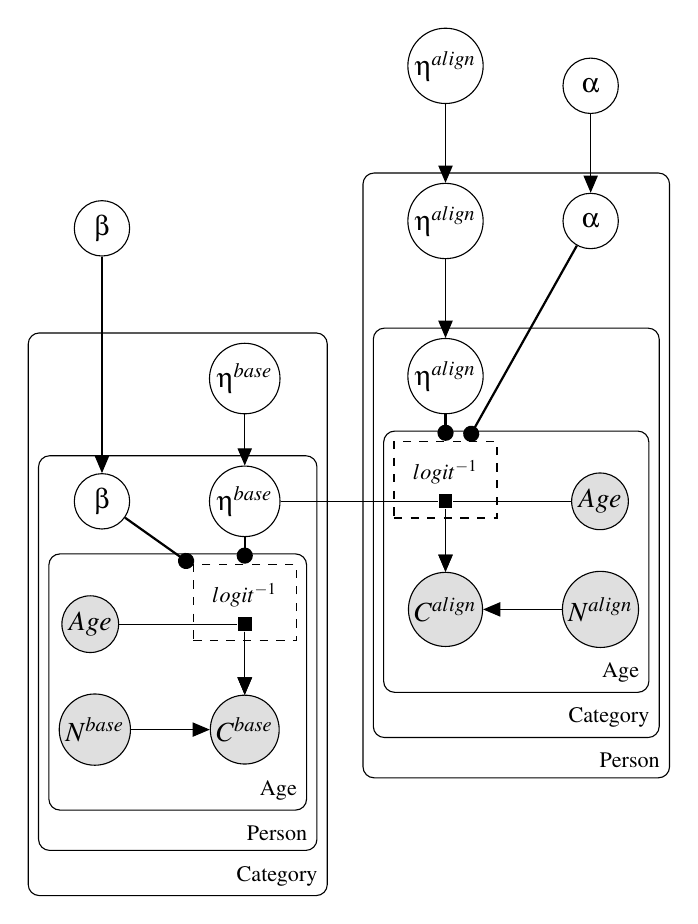
\begin{tikzpicture}[x=1cm,y=1cm]
  
        \node[obs, ]   (C_align)   {$C^{align}$}; %
        \node[obs, right = of C_align]   (N_align) {$N^{align}$}; %
         \node[latent, above = 2 of C_align]   (eta_align_c)   {$\eta^{align}$}; %
         \node[latent, above = of eta_align_c]   (eta_align_p)   {$\eta^{align}$}; %
        \node[latent, above = of eta_align_p]   (eta_align)   {$\eta^{align}$}; %
 	 \factor[above = 0.8 of C_align]       {C_align-f} {$logit^{-1}$} {} {}; %
      
               
          \node[latent, right = of eta_align_p] (age_align_p) {$\alpha$};
          \node[latent, above = of age_align_p] (age_align) {$\alpha$};
      
      
         \gate {logit_align} {(C_align-f)(C_align-f-caption)} {eta_align_c, age_align_p} ; %
         
          \node[obs, right =  1.5 of C_align-f] (Age) {$Age$};

      
       % Nodes
        \node[latent, left = 2 of C_align-f]   (eta_base_p)   {$\eta^{base}$}; %
        \node[obs, below = 2 of eta_base_p]   (C_base)   {$C^{base}$}; %
        \node[latent, above = .65 of eta_base_p]   (eta_base_c)   {$\eta^{base}$}; %
%        \node[latent, above = of eta_base_p]   (eta_base)   {$\eta^{base}$}; %
        \factor[above = 0.8 of C_base]       {C_base-f} {$logit^{-1}$} {} {}; %
        \node[obs, left = of C_base]   (N_base) {$N^{base}$}; %

          \node[obs, left =  1.5 of C_base-f] (Age_base) {$Age$};
      
        \edge{C_base-f}{C_base};
      %  \factoredge {age_align_p} {C_align-f} {C_align} ; 
        \factoredge {Age} {C_align-f} {C_align} ; 
         \factoredge {Age_base} {C_base-f} {C_base} ; 
         
        \node[latent, left = of eta_base_p] (beta_p) {$\beta$};
        \node[latent, above = 2.75 of beta_p] (beta) {$\beta$};

        \edge{eta_base_c}{eta_base_p};
        \edge{age_align}{age_align_p};
  %      \edge{eta_base}{eta_base_p};
        
        \edge{eta_align_p}{eta_align_c};
        \edge{eta_align}{eta_align_p};
        
         \edge{beta}{beta_p};

        \edge {N_base} {C_base};
        \edge {N_align} {C_align};
	 \edge{C_base-f}{C_base};
	 
        \gate {logit_base} {(C_base-f)(C_base-f-caption)} {eta_base_p,beta_p} ; %

        
        \factoredge {eta_base_p} {C_align-f} {C_align} ; %

	\plate {plate_a} {(C_align)(C_align-f)(N_align)(logit_align)(Age)} {Age}; %
	\plate {plate_c} {(C_align)(eta_align_c)(C_align-f)(N_align)(logit_align)(Age)(plate_a)} {Category}; %



	\plate {} {(eta_align_c)(C_align-f)(logit_align)(eta_align_p)(plate_c)(C_align)(N_align)(age_align_p) (Age)(plate_a)}{Person}; %

	
	\plate {plate_a_base} {(C_base)(C_base-f)(N_base)(logit_base)} {Age}; %
	\plate {plate_p_base} {(beta_p)(C_base)(eta_base_p)(C_base-f)(N_base)(logit_base)(plate_a_base)} {Person}; %
	\plate {} {(eta_base_c)(C_base-f)(logit_base)(eta_base_p)(plate_p_base)(C_base)(N_base)(plate_a_base)(eta_base_p)} {Category}; 

\end{tikzpicture}
  \end{center}
  \caption{The Hierarchical Alignment Model (HAM) we use to analyze linguistic alignment in CHILDES. Speaker's word choices are modeled as having two influences: (1) Their baseline probability of using each word category ($\eta_{base}$), and (2) their increase from baseline due to their conversational partner's use of each category in the previous utterance ($\eta_{align}$). }
  \label{fig:model}
\end{figure}

The linguistic tuning hypothesis predicts that parents should tune the complexity of their language to the developing cognitive and linguistic capacities of their children. It thus predicts that parents should show high alignment to their young children, but should gradually reduce their levels of alignment as children develop. To test this hypothesis, we extended the Hierarchical Alignment Model introduced by \citeA{doyle2016}. Our model estimates the extent to which a speaker's use of function words is influenced by their conversational partner's use of words in the same category. In Mom's first response to Naima, for instance, she uses the quantifier ``some'' and the indefinite pronoun ``this'' (Table~\ref{tab:naima}). Would Mom have been less likely to use these words if Naima had not produced a quantifier and an indefinite pronoun in her previous utterance? And would she be less likely if Naima were older?

The model attempts to predict on an utterance-by-utterance level whether a speaker will produce a word belonging to each of the 14 function word categories. The probability of producing a word is controlled by two independent factors: (1) the speaker's baseline probability of producing that word, and (2) the speaker's tendency to align to their conversational partner, producing words from categories that their partner just produced. Thus, the primary computation in the model is essentially the same as standard logistic regression, which predicts a binary response (production) from a linear combination of predictors (word frequency and alignment probability). The remaining machinery of the model allows frequency and alignment estimates to be pooled hierarchically across categories, speakers, and ages in a principled way.

\begin{table}[tb]
\centering
\begin{tabular}{|c|c|c|c|} \hline
Category & Examples & Adult & Child\\ \hline
Article & \textit{a, an, the} & .31 & .13 \\
Certainty  & \textit{always, never} & .05 & .01 \\
Conjunction  & \textit{but, and, though} & .22 & .06\\
Discrepancy  & \textit{should, would} & .11 & .04 \\
Exclusive  & \textit{without, exclude} & .12 & ..04\\
Inclusive  & \textit{with, include} & .21 & .07\\
Indefinite pronoun & \textit{with, include} & .45 & .19\\
Negation   & \textit{not, never} & .21 & .11\\
Preposition& \textit{to, in, by, from}  & .38 & .14\\
Quantifier   & \textit{few, many} & .13 & .04\\
Tentative & \textit{maybe, perhaps} & .11 & .03\\
1st person singular  & \textit{I, me, mine} & .05 & .04\\
1st person plural & \textit{we, us, ours} & .09 & .02\\
2nd person pronoun   & \textit{you, yourself} & .33 & .06\\
\hline
\end{tabular}
\caption{LIWC categories for estimating linguistic alignment, with examples and production probabilities for both adults and children in CHILDES.}\label{tab:LIWC}
\end{table}


\subsection{Model Details}

The full graphical representation of our model is shown in Figure~\ref{fig:model}. The model operates over a representation of utterances as binary vectors indicating the presence or absence of each of the 14 LIWC categories. The probability of producing each category in each utterance is then predicted via two parameters: (1) The speaker's baseline probability for using that word category ($\eta^{base}$), and (2) The speaker's change from this baseline due to interacting with the listener ($\eta^{align}$). For replies to utterances not containing a category, the category's parameter is produced by taking the inverse logit of its baseline log odds $\left(logit^{-1}\left(\eta^{base}\right)\right)$. If the utterance follows an utterance that contains the category, we say that its probability of production is the inverse logit of the sum of the baseline and alignment log odds $\left(logit^{-1}\left(\eta^{base} + (\eta^{align}\right)\right)$.

Because the LIWC categories vary widely in the production frequencies, we draw the log odds of each from an independent uninformative prior $\left(Uniform\left(-5,5\right)\right)$, which covers more than the range of observed probabilities without putting too much mass on extremely large or small values. We put a conservative prior on alignment, drawing $\eta^{align} \sim Normal(0,.5)$, regularizing it strongly towards zero.

To pool data across participants for robust estimation, we estimate all parameters hierarchically. We say that there is a population-level of alignment, which generates speaker-levels of alignment, which generate category-levels of alignment. This decision allows us to make principled inferences both about how much parents align to their children in general, and about how much specific parents align to their children. For baseline probabilities, we instead nest people within categories as the empirical baseline production probabilities vary widely across categories.

Finally, we let both the probability of using any of these categories ($\beta$), and the probability of aligning ($\alpha$) vary over development. Inspection of posterior parameter estimates in a model with independent age estimates showed a linear relationship for both in this age range, so for simplicity we model $\beta$ and $\alpha$ as linear scalars of $\eta^{base}$ and $\eta^{align}$ respectively.

Using this model, we can test two distinct hypotheses about the way that parents might coordinate to their children's developmental level. First, if $\beta$ is non-zero, then we can infer that speakers change their baseline likelihood of producing the function words in the 14 LIWC categories over the course of children's development. If parents' $\beta$ is positive, they are using simpler words earlier in development. Second, if $\alpha$ is non-zero, then we can infer that speakers change their level of alignment over development. If parents' $\alpha$ is negative, they are aligning more to their younger children.

\section{Analysis}

\subsection{Data}

To maximize the power and generalizability of our analysis, we selected all English-language transcripts available in CHILDES containing conversations between a parent and a target child who was 12--60-mos. of age \cite{macwhinney2000}. This yielded  3,851 total transcripts across 417 unique children. The number of transcripts per child varied widely, ranging from 1 ($n = 164$) to 440 ($n = 1$), with a median of 26.

For each transcript, we first combined all successive utterances from the same speaker into one utterance. We then transformed each utterance into a binary vector with a value for each of the 14 LIWC categories \cite{pennebaker2007}. We then formatted the utterances as a series of message-reply pairs, in which each utterance was treated as a reply to the previous utterance, and a message for the next utterance.

\subsection{Method}

For each pair of speakers $A$ and $B$ in a transcript, we computed four counts for each of the 14 LIWC categories: The number messages from $A$ to $B$ containing the category ($N^{align}$), the number of messages from $A$ to $B$ not containing the category ($N^{base}$), the number of replies containing the category to messages containing the category ($C^{align}$), and the number of replies containing the category to messages not containing the category ($C^{base}$). To generate robust parameter estimates, we aggregated counts across all transcripts for the same parent and child into six-month age bins, yielding 8 bins (youngest: 12--18 mo., oldest 54--60 mo.). When estimating $\alpha$ and $\beta$---the age-related scalars---we numbered these bins from 1 to 8 and then subtracted the mean bin number from each (4.5). This centers the intercept ($\eta^{align}$) at the middle value, yielding the smallest average predictive error for other age bins.

We then fit the Hierarchical Alignment Model to the data separately for children and adults. Posterior distributions for all parameters were estimated using a Hamiltonian Monte Carlo sampler \cite{carpenter2016} with three independent chains, and 500 samples in each chain. The first 100 samples of each chain were discarded to ensure sufficient burnin based on inspection of trace plots that typically showed convergence after 50--75 samples. In addition, to provide a baseline for comparison, we also estimated alignment for the parent-parent interactions in the corpus. All data and analysis code are available in a public github repostory at {\small\tt http://github.com/langcog/alignment}.
% Because these were quite sparse relative to parent-child interactions, and because we had no \emph{a priori} reason to expect that parents would align differently to each-other over their children's development, they were not separated into distinct age bins.

\subsection{Results and Discussion}

\begin{figure}[tb]
 \center{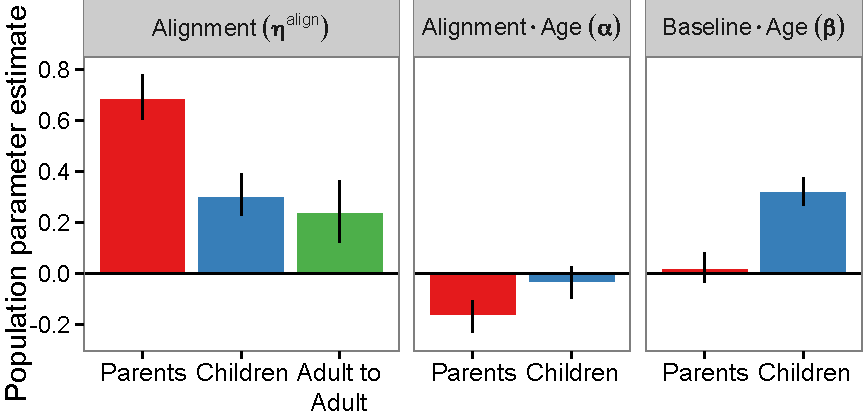
\includegraphics[width=.49\textwidth]{figures/model_params.pdf}}
  \caption{\label{fig:model_parameters} Posterior parameter estimates for alignment ($\eta^{align}$), developmental change in alignment ($\alpha$), developmental change in baseline function word production ($\beta$) for both parents and children, as well estimated estimated alignment between parents for a baseline. Bars indicate means, error-bars indicate  95\% highest posterior density intervals.}
\end{figure}

% The transcripts in CHILDES span a wide range of typical childhood activities---book reading, toy play, dinner, etc. In all of these activities, however, parents and their children use language for common purpose: to communicate. Because successful communication is facilitated by linguistic alignment,  we predict that both parents and their children show reliably positive levels of alignment.

Overall, alignment parameter estimates were above zero for both parents and children, suggesting that both groups aligned (Figure~\ref{fig:model_parameters}). Parents aligned reliably more to their children than children aligned to parents, and parents also aligned reliably more to their children than to each other. Thus, in the aggregate, we can conclude that parents coordinate to their children more than they coordinate to other adults.
% This finding is in line with other work showing that child-directed speech is different from adult-directed speech.

The linguistic tuning hypothesis makes two predictions. First, parents might change the words they produce, using simpler words with younger children. If so, we would expect an increase in their likelihood of producing optional function words (positive $\beta$). In line with previous analyses, we find no evidence of this \cite{newport1977, hayes1988}. (We do, however, find a large and reliable increase in \emph{children's} use of these words as they grow older, as would be expected based on their developing linguistic competence.)

Second, parents could use the same words, but be less contingent on children's production---repeating less, clarifying less, rephrasing less. This second prediction is precisely what we observe in both the aggregate parameter estimates and the developmental parameter estimates (Figure~\ref{fig:all_hpds}). Parental alignment decreases reliably over development, and children's alignment shows a similar trend. Thus, parent-child conversations become gradually less coordinated over development, settling to the adult-adult baseline as children need less scaffolding to be successful communicators.


\begin{figure}[tb]
 \center{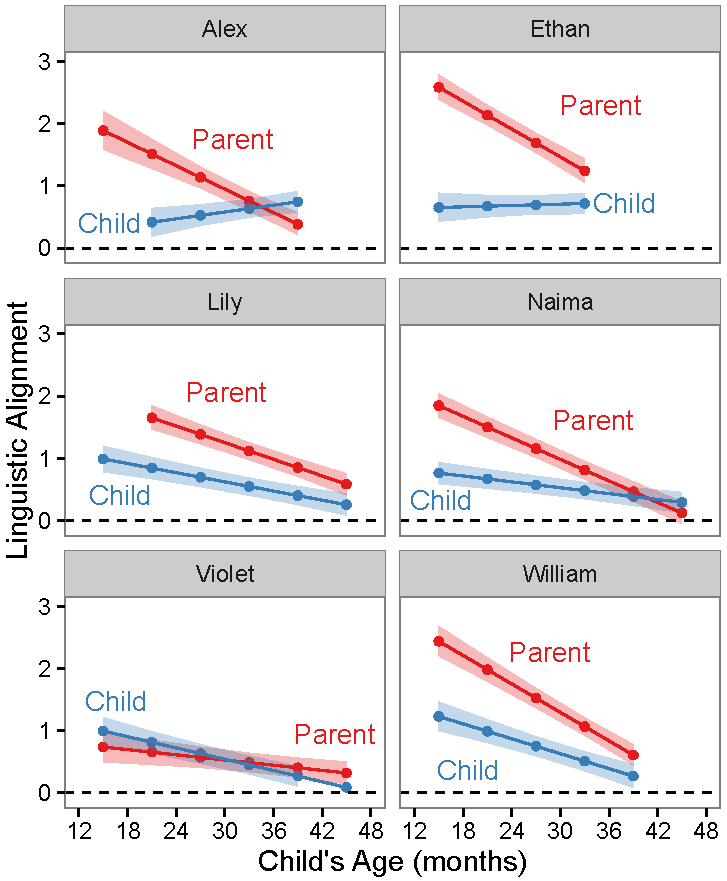
\includegraphics[width=.48\textwidth]{figures/providence_hpds.pdf}}
  \caption{\label{fig:providence_hpds} Changes in alignment for 6 children and their parents measured longitudinally in the Providence corpus \cite{demuth2006}. Points indicate the mean of the posterior distribution, shaded regions indicate 68\% highest probability density intervals.}
\end{figure}

\begin{figure*}[tb]
	\center{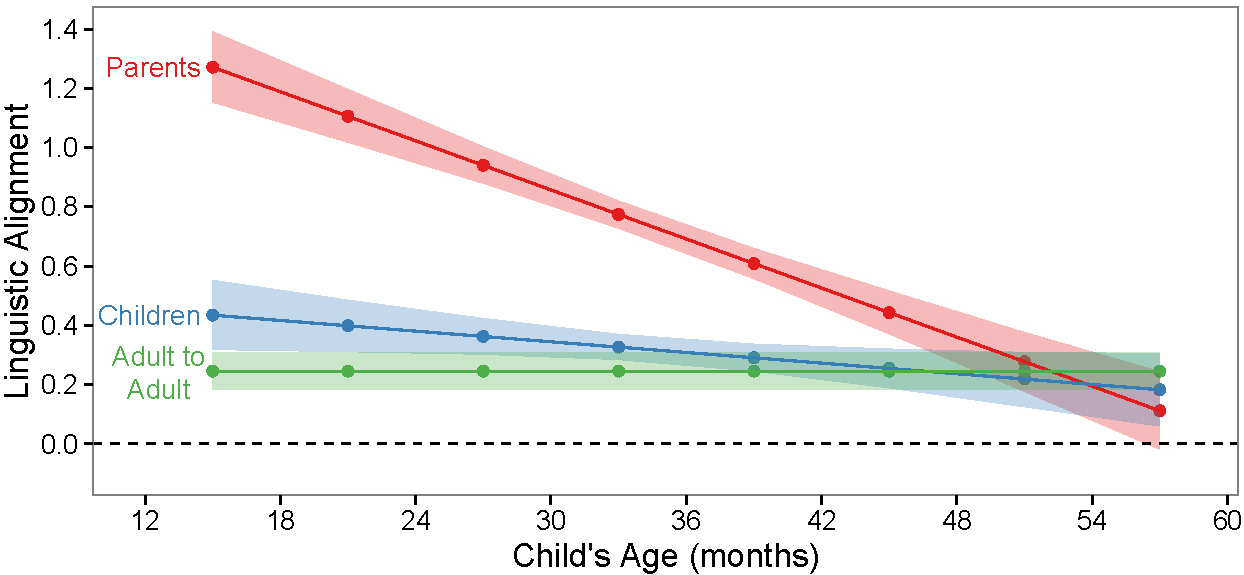
\includegraphics[width=.95\textwidth]{figures/all_hpds.pdf}}
	\caption{Model-estimated changes in linguistics alignment by 6-month-window. Over development, both parents and children decrease in their linguistic alignment to each other until they align at adult-adult levels. Points indicate the mean of the posterior distribution, shaded regions indicate 68\% highest probability density intervals, equivalent to one standard deviation.
\label{fig:all_hpds} }
\end{figure*}

In addition to estimating population-level parameters for alignment and its change over development, our hierarchical model also estimates parameters for each of the individual adults and children in CHILDES. Examining these parameters shows both consistency and variability across dyads (Figure~\ref{fig:providence_hpds}). Across children, parental alignment is consistently highest early in development, but both children and parents vary in their level of alignment and in the rate at which it changes across development. These reliable individual differences in alignment present a possible vehicle for studying individual differences in children's language acquisition.
\vspace{6pt}

\subsubsection{LIWC Category Validation Control.}

Our measure of alignment is sensitive to repetitions, reformulations, expansions, and other conversational turns that result in contingency of function word categories. But, the alignment we observed in parent-child interactions could driven entirely by repetition. To control for this, we constructed a set of shuffled LIWC categories by randomly permuting the original word-category assignments. If these shuffled categories yield the same levels of alignment as the original categories, we would conclude that linguistic alignment between parents and children is happening at the word level rather than the category level. Compared to 40 different random shuffles, parents' alignment on the original categories ($\eta^{align}$) was greater than 37, and developmental change in alignment ($\alpha$) was greater than all 40 ($p < .001$). Similarly, children's on the LIWC categories was greater than all 40 shuffled categories ($p < .001$). Thus, the developmental changes in alignment we observed are not just due to more exact repetitions in early childhood, but also higher-level linguistic coordination.

\section{General Discussion}

Although even the youngest infants are equipped with the capacity to learn from the language they hear, their learning is highly constrained by their developing attentional and memory systems \cite{vlach2013}. How do children acquire language so rapidly despite these cognitive constraints? One hypothesis is that the the language they hear is tuned to their learning capacities, providing the right kind of information at the right time \cite{snow1972, vygotsky1978}.

Previous attempts to test this hypothesis have produced a mixture of evidence, with some in strong support of the linguistic tuning hypothesis \cite<e.g.>{hirsh-pasek1984, chouinard2003}, others in strong opposition \cite<e.g.>{brown1970, newport1977}, and yet others finding mixed support and interesting individual differences \cite<e.g.>{sokolov1993, dale2006}. Our work leverages the power of hierarchical Bayesian models to integrate together data from two orders of magnitude more children than previous work, providing a more robust test of tuning.

We find, at the population level, that parents indeed provide linguistic input that is calibrated to children's development. The structural elements of their utterances are strongly contingent on children's previous productions early in development, but gradually approach adult-adult levels of coordination. In line with previous work, we do not find evidence of change at a global level: Parents do not use different words when talking to children of different ages \cite{hayes1988}. Instead, calibration is local---sensitive to the on-going conversation and attuned to children's processing in context.
% This is consonant with a number of previous studies showing that children's distributional learning is powerful at short time-scales, but falls off over long intervals \cite{onnis2008, goldstein2010}.


% Although the nature of the data in CHILDES does not allow us to discover either the sources of the consequences of the individual differences, they suggest a promising future direction for understanding the incredible variation in children's language acquisition.


% The titration of difficulty to developmentally appropriate levels may be precisely the structure that is ideal for children's children's learning \cite{elman1993, fausey2016}.

As opposed to across-the-board simplification, linguistic tuning may be particularly beneficial for learning. Because context provides so much support for children's comprehension, perhaps the best thing that parents can do is provide support in context. Critically, linguistic tuning does not require that parents consciously have as their goal the optimization of children's learning. They need not be teachers; they need only be communicators. If parents want to communicate with their children, and their children need significant linguistic support, they will have no choice but to align.

\section{Acknowledgments}

We are grateful to Aaron Chuey and Jake Prasad for help with an earlier version of the model. This work was supported by NIH NRSA F32HD075577 to DY and NSF BCS\#1528526 and \#1456077 to MCF.


\bibliographystyle{myapacite}

\setlength{\bibleftmargin}{.125in}
\setlength{\bibindent}{-\bibleftmargin}

\bibliography{alignment}


\end{document}
